\documentclass[10pt,aspectratio=169]{beamer}
\usepackage[utf8]{inputenc}
\usepackage[T1]{fontenc}
\usepackage[french]{babel}
\usepackage{graphicx}
\usepackage{xcolor}
\usepackage{tikz}
\usepackage{amsmath,amsfonts,amssymb}
\usepackage{booktabs}
\usepackage{tabularx}
\usepackage{tcolorbox}
\usepackage{tikz}

% Configuration des bibliothèques TikZ nécessaires pour les diagrammes
\usetikzlibrary{shapes.geometric, arrows.meta, positioning, fit, backgrounds, shapes.multipart}

% Couleurs personnalisées (identiques au mémoire)
\definecolor{insiturquoise}{RGB}{45,140,130}
\definecolor{insinavy}{RGB}{25,50,75}
\definecolor{insidarkblue}{RGB}{20,40,65}
\definecolor{insilightbg}{RGB}{248,249,250}

% Configuration du thème Beamer
\usetheme{default}
\usefonttheme{serif} % Utilisation de polices serif plus académiques
\usecolortheme{default}

% Personnalisation des éléments Beamer
\setbeamercolor{title}{fg=insinavy}
\setbeamercolor{frametitle}{fg=insinavy, bg=insilightbg}
\setbeamercolor{structure}{fg=insinavy}
\setbeamercolor{item}{fg=insiturquoise}
\setbeamercolor{block title}{bg=insinavy, fg=white}
\setbeamercolor{block body}{bg=insilightbg, fg=black}
\setbeamercolor{block title example}{bg=insiturquoise, fg=white}
\setbeamercolor{block body example}{bg=insilightbg, fg=black}

% Suppression des symboles de navigation pour une présentation épurée
\setbeamertemplate{navigation symbols}{}

% Configuration du pied de page
\setbeamertemplate{footline}{%
  \begin{beamercolorbox}[wd=\paperwidth,ht=2.5ex,dp=1.125ex,leftskip=1.5em,rightskip=1.5em]{palette tertiary}%
    \color{gray}\usebeamerfont{footline}%
   \hfill \insertframenumber/\inserttotalframenumber
  \end{beamercolorbox}%
}

% Page de titre personnalisée
\title[\textbf{Restructuration Backend}]{\textbf{RESTRUCTURATION DU BACKEND D'UNE PLATEFORME E-COMMERCE}}
\subtitle{Transition d'un Monolithe vers une Architecture Microservices}
\author[\textbf{T. RATOLOJANAHARY}]{\textbf{Monsieur RATOLOJANAHARY Tina Hubert}}
\institute[INSI]{\textbf{INSI UNIVERSITY} \\ Institut National Supérieur d'Informatique \\ Parcours : MSI (Master 2)}
\date[Soutenance 2026]{Année universitaire : 2024--2025}

\begin{document}

% --- SLIDE 1 : TITRE ---
\begin{frame}[plain]
    \begin{center}
        
\includegraphics[width=2.5cm]{insilogo.png} \\[1ex]
        {\small\color{gray}\textbf{INSI}} \\[1ex]
        \centerline{\rule{4cm}{0.4pt}}
        \vspace{2ex}
        {\usebeamercolor[fg]{title}\usebeamerfont{title}\Large\inserttitle} \\
        {\color{insiturquoise}\large\insertsubtitle} \\[2ex]
        
        \begin{tcolorbox}[colback=insinavy, colframe=insinavy, arc=2mm, width=0.85\linewidth, center]
            \centering\color{white}\small
            Mémoire de projet présenté en vue de l'obtention du diplôme de Master 2
        \end{tcolorbox}
        
        \vspace{2ex}
        \begin{tabular}{cc}
            \textbf{Présenté par :} & \textbf{Sous la direction de :} \\
            Tina Hubert RATOLOJANAHARY & Membres du Jury de l'INSI
        \end{tabular}
    \end{center}
\end{frame}

% --- SLIDE 2 : SOMMAIRE ---
\begin{frame}{\textbf{Sommaire de la Présentation}}
    \begin{columns}
        \begin{column}{0.5\textwidth}
            \begin{block}{\textbf{Introduction et Contexte}}
                \begin{itemize}
                    \item Contexte et Problématique
                    \item Objectifs de la Migration
                \end{itemize}
            \end{block}
            \begin{block}{\textbf{Conception et Choix Techniques}}
                \begin{itemize}
                    \item Modélisation DDD et Découpage
                    \item Communication Inter-services (RabbitMQ)
                    \item Persistance Polyglotte et Pattern Saga
                \end{itemize}
            \end{block}
        \end{column}
        \begin{column}{0.5\textwidth}
            \begin{block}{\textbf{Réalisation Technique}}
                \begin{itemize}
                    \item Structure Monorepo et NestJS
                    \item API Gateway et Sécurisation
                    \item Tracing avec Jaeger et Observabilité
                \end{itemize}
            \end{block}
            \begin{block}{\textbf{Résultats et Conclusion}}
                \begin{itemize}
                    \item Bilan des Performances (Artillery)
                    \item Analyse Statistique du Code (Lizard, LOC)
                    \item Perspectives et Améliorations Futures
                \end{itemize}
            \end{block}
        \end{column}
    \end{columns}
\end{frame}

% ==========================================
% SECTION 1 : INTRODUCTION
% ==========================================
\section{Introduction}

% --- SLIDE 3 : CONTEXTE ---
\begin{frame}{\textbf{Contexte du Projet : Plateforme Techcare}}
    \begin{columns}
        \begin{column}{0.6\textwidth}
            \begin{itemize}
                \item \textbf{Techcare} : Plateforme e-commerce officinale pour la vente en ligne de médicaments et produits de santé.
                \item \textbf{Le Point de Départ} : Une application monolithique traditionnelle construite en JavaScript/Node.js.
                \item \textbf{Le Défi} : Assurer la transition d'un monolithe vers une architecture orientée microservices moderne sans rupture de service et en garantissant la cohérence.
            \end{itemize}
        \end{column}
        \begin{column}{0.4\textwidth}
            \begin{block}{\textbf{Architecture Initiale}}
                \begin{itemize}
                    \item Base de code unique
                    \item Base de données relationnelle unique
                    \item Couplage fort entre fonctions
                \end{itemize}
            \end{block}
        \end{column}
    \end{columns}
\end{frame}

% --- SLIDE 4 : PROBLEMATIQUE ---
\begin{frame}{\textbf{Problématique du Monolithe Legacy}}
    \begin{columns}
        \begin{column}{0.5\textwidth}
            \begin{alertblock}{\textbf{Limites Techniques et Organisationnelles}}
                \begin{itemize}
                    \item \textbf{"Big Ball of Mud"} : Code difficilement maintenable avec un risque élevé de régression.
                    \item \textbf{Déploiements bloquants} : Une seule correction nécessite le redéploiement complet.
                    \item \textbf{Absence de Scalabilité Ciblée} : Impossible de scaler le module de catalogue sans dupliquer la gestion des paiements.
                    \item \textbf{SPOF (Single Point of Failure)} : Un crash mémoire dans un module paralyse toute la pharmacie.
                \end{itemize}
            \end{alertblock}
        \end{column}
        \begin{column}{0.5\textwidth}
            \begin{block}{\textbf{Objectifs de la Migration}}
                \begin{itemize}
                    \item \textbf{Isolation des pannes} (Résilience).
                    \item \textbf{Scalabilité horizontale sélective}.
                    \item \textbf{Indépendance des cycles de livraison}.
                    \item \textbf{Charge cognitive réduite} par service.
                \end{itemize}
            \end{block}
        \end{column}
    \end{columns}
\end{frame}

% ==========================================
% SECTION 2 : CONCEPTION
% ==========================================
\section{Conception et Architecture}

% --- SLIDE 5 : DDD ---
\begin{frame}{\textbf{Découpage Métier : Le Domain-Driven Design (DDD)}}
    \begin{columns}
        \begin{column}{0.5\textwidth}
            \begin{itemize}
                \item Analyse approfondie des domaines métiers pour définir des \textbf{Bounded Contexts} (contextes délimités).
                \item Chaque microservice possède sa propre responsabilité métier claire.
                \item Utilisation de l'**Ubiquitous Language** (ex: \texttt{RESERVATION}/\texttt{RELEASE}, \texttt{stock\_unavailable}) directement dans le code pour aligner technique et métier.
            \end{itemize}
        \end{column}
        \begin{column}{0.5\textwidth}
            \begin{block}{\textbf{Les Contextes Retenus}}
                \begin{description}
                    \item[Product Manager] Catalogue de médicaments (NoSQL)
                    \item[Inventory Manager] Gestion fine des stocks (ACID)
                    \item[Order Manager] Gestion des paniers et commandes
                    \item[User Manager] Authentification et rôles (RBAC)
                    \item[Support Services] File Manager, Payment, Notification
                \end{description}
            \end{block}
        \end{column}
    \end{columns}
\end{frame}

% --- SLIDE 6 : DOCKER COMMUNICATION ---
\begin{frame}{\textbf{Architecture des Conteneurs et Communications}}
    \begin{center}
        \resizebox{!}{0.7\textheight}{
            \begin{tikzpicture}[
    node distance=1.2cm and 1.5cm,
    box/.style={
        draw=gray!50,
        fill=white,
        rounded corners=3pt,
        minimum width=3.8cm,
        minimum height=0.75cm,
        align=center,
        font=\small\sffamily
    },
    bluebox/.style={
        draw=blue!50!cyan,
        fill=blue!5,
        rounded corners=3pt,
        minimum width=4.5cm,
        minimum height=0.9cm,
        align=center,
        font=\bfseries\small\sffamily
    },
    purplebox/.style={
        draw=violet!60,
        fill=violet!5,
        rounded corners=3pt,
        minimum width=4.0cm,
        minimum height=0.8cm,
        align=center,
        font=\bfseries\small\sffamily
    },
    cloudbox/.style={
        draw=violet!60,
        fill=violet!5,
        dashed,
        rounded corners=3pt,
        minimum width=5.0cm,
        minimum height=0.9cm,
        align=center,
        font=\bfseries\small\sffamily
    },
    dbshape/.style={
        cylinder,
        draw=violet!60,
        fill=violet!5,
        minimum width=2.6cm,
        minimum height=1.0cm,
        shape border rotate=90,
        aspect=0.25,
        align=center,
        font=\bfseries\small\sffamily
    },
    frame/.style={
        draw=gray!40,
        fill=yellow!5,
        rounded corners=6pt,
        inner sep=12pt
    },
    outerframe/.style={
        draw=yellow!60!olive,
        fill=yellow!3,
        rounded corners=8pt,
        inner sep=15pt
    }
]

    % Nodes Placement
    
    % Client (outside infrastructure)
    \node[purplebox] (client) at (0, 10.5) {Client (Frontend)};
    
    % Infrastructure Docker elements
    \node[bluebox] (gateway) at (0, 8.0) {API Gateway (NestJS)};
    \node[bluebox] (rabbitmq) at (0, 5.5) {RabbitMQ Broker};
    
    % Services Métier (Left Column)
    \node[box] (user) at (-3.5, 2.0) {user-manager};
    \node[box] (product) at (-3.5, 1.0) {product-manager};
    \node[box] (cart) at (-3.5, 0.0) {cart-manager};
    \node[box] (order) at (-3.5, -1.0) {order-manager};
    \node[box] (inventory) at (-3.5, -2.0) {inventory-manager};
    
    % Services Support (Right Column)
    \node[box] (file) at (3.5, 1.7) {file-manager};
    \node[box] (payment) at (3.5, 0.7) {payment-manager};
    \node[box] (notification) at (3.5, -0.3) {notification-manager};
    \node[box] (jaeger) at (3.5, -1.3) {jaeger (Tracing)};
    
    % Persistance (Bottom)
    \node[dbshape] (postgres) at (-1.5, -4.5) {PostgreSQL};
    \node[dbshape] (mongodb) at (1.5, -4.5) {MongoDB};
    
    % External Services (Outside Docker at the bottom)
    \node[cloudbox] (external) at (0, -7.5) {Services Cloud Externes\\(AWS S3 / Stripe)};

    % Background Frames (Ordered from back to front)
    \begin{scope}[on background layer]
        % 1. Outer Frame (Infrastructure Docker)
        \node[outerframe, fit=(gateway) (rabbitmq) (user) (inventory) (file) (jaeger) (postgres) (mongodb),
              label={[anchor=south west, font=\bfseries\sffamily, text=olive!90!black, xshift=12pt, yshift=2pt]north west:Infrastructure Docker}] (docker_frame) {};
        
        % 2. Microservices Layer Box (Middle Frame)
        \node[draw=yellow!80!olive!70, fill=yellow!8, rounded corners=6pt, inner sep=16pt, fit=(user) (inventory) (file) (jaeger),
              label={[anchor=south, font=\bfseries\small\sffamily, text=olive!90!black, yshift=2pt]above:Microservices Layer}] (ms_layer_frame) {};
        
        % 3. Services Métier Box (Inner Frame Left)
        \node[frame, fit=(user) (inventory),
              label={[anchor=south west, font=\bfseries\small\sffamily, text=olive!80!black, xshift=8pt, yshift=2pt]north west:Services Métier}] (metier_frame) {};
        
        % 4. Services Support Box (Inner Frame Right)
        \node[frame, fit=(file) (jaeger),
              label={[anchor=south west, font=\bfseries\small\sffamily, text=olive!80!black, xshift=8pt, yshift=2pt]north west:Services Support}] (support_frame) {};
        
        % 5. Persistance Box (Inner Frame Bottom)
        \node[frame, fit=(postgres) (mongodb),
              label={[anchor=south west, font=\bfseries\small\sffamily, text=olive!80!black, xshift=8pt, yshift=2pt]north west:Persistance (Bases)}] (persistance_frame) {};
    \end{scope}

    % Connections
    
    % Client -> Gateway
    \draw[-{Stealth[scale=1.2]}, thick] (client) -- node[fill=white, draw=gray!30, rounded corners=2pt, font=\scriptsize\sffamily, inner sep=2pt] {HTTP/REST} (gateway);
    
    % Gateway -> RabbitMQ
    \draw[-{Stealth[scale=1.2]}, thick] (gateway) -- node[fill=white, draw=gray!30, rounded corners=2pt, font=\scriptsize\sffamily, inner sep=2pt] {RPC} (rabbitmq);
    
    % RabbitMQ <-> Services Métier
    \draw[{Stealth[scale=1.0]}-{Stealth[scale=1.0]}, thick] (rabbitmq.south west) to[out=210, in=90] (metier_frame.north);
    
    % RabbitMQ <-> Services Support
    \draw[{Stealth[scale=1.0]}-{Stealth[scale=1.0]}, thick] (rabbitmq.south east) to[out=330, in=90] (support_frame.north);
    
    % Services Métier -> Persistance
    \draw[thick] (metier_frame.south) to[out=270, in=135] (persistance_frame.north west);
    
    % Services Support -> Persistance
    \draw[thick] (support_frame.south) to[out=270, in=45] (persistance_frame.north east);
    
    % Services Support -> External Cloud Services
    \draw[thick, dashed, -{Stealth[scale=1.0]}] (support_frame.south) to[out=290, in=45] (external.north east);

\end{tikzpicture}

        }
    \end{center}
\end{frame}

% --- SLIDE 7 : PERSISTANCE POLYGLOTTE ---
\begin{frame}{\textbf{Persistance Polyglotte : Le bon outil au bon endroit}}
    Le choix des bases de données répond à des impératifs techniques divergents :
    
    \vspace{2ex}
    \begin{table}
        \centering
        \renewcommand{\arraystretch}{1.3}
        \begin{tabularx}{\textwidth}{l X X}
            \toprule
            \textbf{Critère} & \textbf{PostgreSQL (Inventory/Orders)} & \textbf{MongoDB (Product Catalog)} \\
            \midrule
            \textbf{Modèle de données} & Relationnel (Schéma fixe et strict) & Documentaire (Schéma dynamique) \\
            \textbf{Garanties} & Forte cohérence (ACID) & Haute disponibilité (BASE) \\
            \textbf{Cas d'utilisation} & \textbf{Éviter le Double Spending} lors des réservations de stock & Métadonnées hétérogènes (posologie, composition, photos) \\
            \textbf{Bénéfice} & Transactions complexes fiables & Rapidité de consultation et flexibilité \\
            \bottomrule
        \end{tabularx}
    \end{table}
\end{frame}

% --- SLIDE 8 : TRANSACTION ET SAGA ---
\begin{frame}{\textbf{Transactions Distribuées : Pattern Saga par Chorégraphie}}
    \begin{columns}
        \begin{column}{0.5\textwidth}
            \begin{block}{\textbf{Problématique}}
                Chaque microservice ayant sa propre base de données, impossible d'effectuer un commit global ACID en cas d'erreur réseau ou applicative.
            \end{block}
            \begin{block}{\textbf{Solution : Saga Décentralisée}}
                \begin{itemize}
                    \item Enchaînement d'événements asynchrones via RabbitMQ.
                    \item Si une étape échoue (ex: paiement refusé), des \textbf{événements de compensation} sont émis pour annuler les étapes précédentes (ex: libération du stock réservé).
                \end{itemize}
            \end{block}
        \end{column}
        \begin{column}{0.5\textwidth}
            \begin{exampleblock}{\textbf{Déroulement d'une commande}}
                \begin{enumerate}
                    \item validation du produit (NoSQL)
                    \item réservation de stock (PostgreSQL)
                    \item débit bancaire (Stripe)
                    \item confirmation (Email / WS)
                \end{enumerate}
            \end{exampleblock}
        \end{column}
    \end{columns}
\end{frame}

% ==========================================
% SECTION 3 : REALISATION
% ==========================================
\section{Réalisation Technique}

% --- SLIDE 9 : IMPLEMENTATION CORE ---
\begin{frame}{\textbf{Choix Technologiques et Structure du Code}}
    \begin{columns}
        \begin{column}{0.6\textwidth}
            \begin{itemize}
                \item \textbf{TypeScript \& NestJS} : Choix motivé par la rigueur du typage et le design pattern d'injection de dépendances (DI) facilitant l'architecture en couches (Clean/Hexagonal).
                \item \textbf{RabbitMQ} : Utilisé comme Message Broker asynchrone pour propager les événements métiers.
                \item \textbf{Shared Library} : Paquet centralisé hébergeant les DTOs, enums et filtres d'exceptions globaux (RpcExceptionFilter).
            \end{itemize}
        \end{column}
        \begin{column}{0.4\textwidth}
            \begin{block}{\textbf{Structure du Projet}}
                \texttt{techcare-monorepo/} \\
                \texttt{\quad |-- apps/} \\
                \texttt{\quad | \quad |-- api-gateway/} \\
                \texttt{\quad | \quad |-- order-manager/} \\
                \texttt{\quad | \quad +-- ... (autres services)} \\
                \texttt{\quad +-- libs/} \\
                \texttt{\quad \quad  +-- shared/}
            \end{block}
        \end{column}
    \end{columns}
\end{frame}

% --- SLIDE 10 : SECURITE & GATEWAY ---
\begin{frame}{\textbf{API Gateway et Sécurisation}}
    \begin{columns}
        \begin{column}{0.5\textwidth}
            \begin{block}{\textbf{Rôle de l'API Gateway}}
                \begin{itemize}
                    \item Point d'entrée unique (BFF).
                    \item Routage des requêtes vers les services.
                    \item Validation centralisée des données (DTOs).
                    \item Détection et interception des exceptions internes.
                \end{itemize}
            \end{block}
        \end{column}
        \begin{column}{0.5\textwidth}
            \begin{block}{\textbf{Sécurité Applicative (Principes Zero Trust)}}
                \begin{itemize}
                    \item Authentification par jeton \textbf{JWT} au niveau de la Gateway.
                    \item propagation de l'identité de l'utilisateur à travers les microservices via les headers de message.
                    \item Contrôle d'accès par rôles (\textbf{RBAC}) sur les endpoints sensibles (Admin vs Client).
                \end{itemize}
            \end{block}
        \end{column}
    \end{columns}
\end{frame}

% --- SLIDE 10b : SCENARIO DE DEMONSTRATION ---
\begin{frame}{\textbf{Scénario de Démonstration Live}}
    \begin{columns}
        \begin{column}{0.5\textwidth}
            \begin{block}{\textbf{Étape 1 : Cycle Nominal (Succès)}}
                \begin{itemize}
                    \item \textbf{Achat Client} : Commande d'un produit.
                    \item \textbf{Coulisses} : Validation $\rightarrow$ Réservation stock $\rightarrow$ Débit Stripe $\rightarrow$ Email.
                    \item \textbf{UI} : Notification temps réel par WebSockets.
                \end{itemize}
            \end{block}
            \begin{block}{\textbf{Étape 2 : Administration \& RBAC}}
                \begin{itemize}
                    \item Requête directe API par le Client (ex: Postman/cURL) $\rightarrow$ Rejetée (403 Forbidden).
                    \item Connexion Admin sur l'interface $\rightarrow$ Ajout produit dans le catalogue MongoDB.
                \end{itemize}
            \end{block}
        \end{column}
        \begin{column}{0.5\textwidth}
            \begin{block}{\textbf{Étape 3 : Transaction de Compensation}}
                \begin{itemize}
                    \item Commande client $\rightarrow$ Débit Stripe échoué.
                    \item Déclenchement de la compensation $\rightarrow$ Libération automatique du stock réservé.
                \end{itemize}
            \end{block}
            \begin{block}{\textbf{Étape 4 : Injection de Panne \& Tracing}}
                \begin{itemize}
                    \item Arrêt forcé d'une base de données ou d'un service.
                    \item Analyse visuelle directe du flux d'erreur dans le tableau de bord \textbf{Jaeger}.
                \end{itemize}
            \end{block}
        \end{column}
    \end{columns}
\end{frame}

% ==========================================
% SECTION 4 : RESULTATS ET ANALYSE
% ==========================================
\section{Résultats et Analyse}

% --- SLIDE 11 : TESTS DE CHARGE ---
\begin{frame}{\textbf{Analyse des Performances sous Stress (Artillery)}}
    \begin{columns}
        \begin{column}{0.5\textwidth}
            Un test de charge de \textbf{5 660 requêtes} sur 4 minutes (jusqu'à 100 requêtes/sec) a mis en évidence le comportement des systèmes :
            \begin{itemize}
                \item \textbf{Latence Nominale (Médiane)} : 29,1 ms pour les microservices contre 7 ms pour le monolithe.
                \item \textbf{"Impôt de la distribution"} : Surcharges liées au réseau (Network Hop), à la sérialisation JSON et au routage Gateway.
                \item \textbf{Résilience au stress} : Taux de succès de \textbf{86,5\%} en microservices en pic de charge extrême (timeouts Gateway).
            \end{itemize}
        \end{column}
        \begin{column}{0.5\textwidth}
            \begin{block}{\textbf{Latence de Queue (p95/p99)}}
                \begin{itemize}
                    \item \textbf{p95} : 2,8 secondes.
                    \item \textbf{p99} : 6,8 secondes.
                    \item Preuve de la saturation des connexions socket en haute charge sans auto-scaling dynamique.
                \end{itemize}
            \end{block}
        \end{column}
    \end{columns}
\end{frame}

% --- SLIDE 12 : QUALITE LOGICIELLE ---
\begin{frame}{\textbf{Qualité Logicielle et Maintenabilité}}
    \begin{columns}
        \begin{column}{0.6\textwidth}
            \begin{itemize}
                \item \textbf{Volume de Code par dépôt} :
                      \begin{itemize}
                          \item Monolithe global : \textbf{8 087 lignes} de code.
                          \item Service Produit isolé : \textbf{716 lignes} (-91\%).
                          \item Charge cognitive drastiquement réduite pour les équipes.
                      \end{itemize}
                \item \textbf{Complexité Cyclomatique (Lizard)} :
                      \begin{itemize}
                          \item Baisse du CCN moyen de \textbf{1,8} à \textbf{1,2}.
                          \item Moins de chemins d'exécution, réduction du risque de bugs logiques.
                      \end{itemize}
            \end{itemize}
        \end{column}
        \begin{column}{0.4\textwidth}
            \begin{block}{\textbf{Indicateurs Lizard}}
                \renewcommand{\arraystretch}{1.2}
                \begin{tabular}{lcc}
                    \toprule
                    \textbf{Métrique} & \textbf{Mono} & \textbf{Micro} \\
                    \midrule
                    Fonctions & 297 & 12 \\
                    \textbf{CCN Moy.} & \textbf{1.8} & \textbf{1.2} \\
                    LOC / fonc. & 15.6 & 3.8 \\
                    \bottomrule
                \end{tabular}
            \end{block}
        \end{column}
    \end{columns}
\end{frame}

% --- SLIDE 13 : JAEGER OBSERVARBILITE ---
\begin{frame}{\textbf{Observabilité et Isolation : Simulation de Panne}}
    \begin{columns}
        \begin{column}{0.5\textwidth}
            \begin{block}{\textbf{Scénario de test : MongoDB Down}}
                Nous avons volontairement coupé MongoDB (catalogue produits) pour évaluer la résilience.
            \end{block}
            \begin{block}{\textbf{Constats}}
                \begin{itemize}
                    \item \textbf{Dégradation Gracieuse} : Le catalogue devient indisponible, mais le reste (Paiements, Commandes) fonctionne.
                    \item \textbf{Observabilité immédiate} : Grâce à \textbf{Jaeger} et \textbf{OpenTelemetry}, la cause (MongoDB Timeout) est identifiée en 2 secondes, sans fouiller les logs textuels de tous les conteneurs.
                \end{itemize}
            \end{block}
        \end{column}
        \begin{column}{0.5\textwidth}
            \begin{center}
                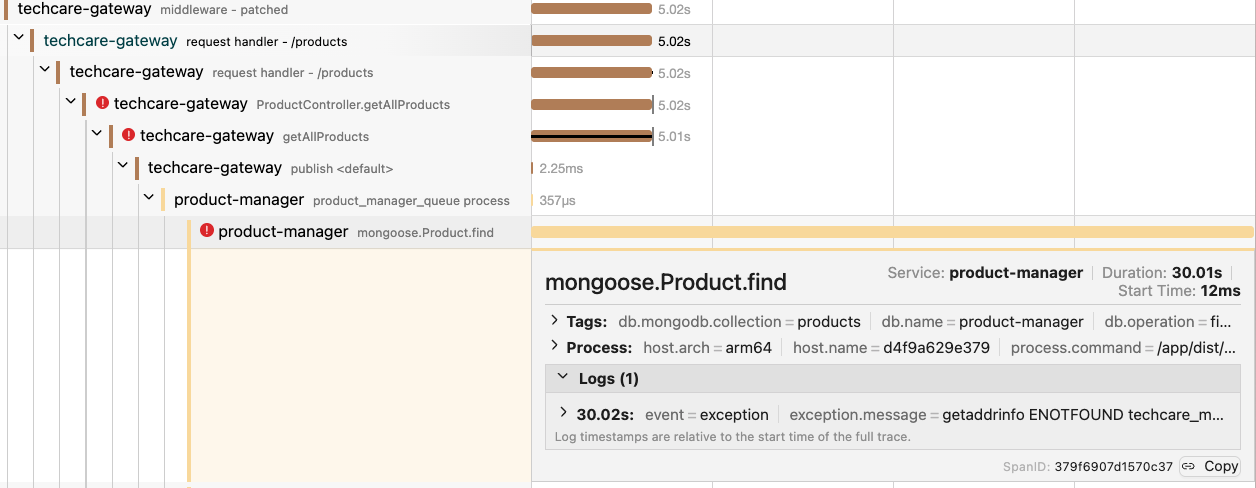
\includegraphics[width=\textwidth]{diagrams/images/jaeger_mongo_down.png}
                \vspace{0.1cm}
                {\scriptsize Trace Jaeger identifiant la défaillance}
            \end{center}
        \end{column}
    \end{columns}
\end{frame}

% --- SLIDE 14 : BILAN SYNTHETIQUE ---
\begin{frame}{\textbf{Bilan Quantitatif Global : Avant vs Après}}
    \renewcommand{\arraystretch}{1.2}
    \small
    \begin{tabularx}{\textwidth}{p{3.8cm} p{5.0cm} p{5.0cm}}
        \toprule
        \textbf{Indicateur} & \textbf{Ancien Monolithe} & \textbf{Nouvelle Architecture} \\
        \midrule
        \textbf{Temps de réponse (Médiane)} & 7 ms (Accès mémoire direct) & 29,1 ms (Réseau + Routage Gateway) \\
        \textbf{Taux de succès sous stress} & 100 \% & 86,5 \% (Saturation socket Gateway) \\
        \textbf{Temps de démarrage (Cache)} & 1,280 s (1 conteneur) & 19,671 s (Orchestration multi-services) \\
        \textbf{Charge cognitive (LOC / dépôt)} & 8 087 lignes (Projet unique) & $\sim$ 700 lignes (Par microservice) \\
        \textbf{Complexité Cyclomatique (CCN)} & 1,8 (Moyenne) & 1,2 (Moyenne - Single Responsibility) \\
        \textbf{Résilience au crash critique} & Effondrement global du système & Dégradation gracieuse (Jaeger identifié) \\
        \bottomrule
    \end{tabularx}
\end{frame}

% ==========================================
% SECTION 5 : PERSPECTIVES & CONCLUSION
% ==========================================
\section{Conclusion}

% --- SLIDE 15 : PERSPECTIVES ---
\begin{frame}{\textbf{Perspectives d'Améliorations Futures}}
    \begin{columns}
        \begin{column}{0.5\textwidth}
            \begin{block}{\textbf{DevOps \& Infrastructure}}
                \begin{itemize}
                    \item \textbf{Kubernetes (K8s)} : Auto-scaling horizontal automatique des pods lors des pics de charge, éliminant les échecs de connexion.
                    \item \textbf{Service Mesh (Istio)} : Sécurité inter-services chiffrée (mTLS) et gestion intelligente du trafic réseau.
                \end{itemize}
            \end{block}
        \end{column}
        \begin{column}{0.5\textwidth}
            \begin{block}{\textbf{Optimisations Applicatives}}
                \begin{itemize}
                    \item \textbf{Cache Redis} : Intégration d'une couche de cache au niveau de l'API Gateway pour faire chuter le temps de réponse de consultation (2 à 5 ms).
                    \item \textbf{gRPC} : Remplacement du HTTP/JSON interne par gRPC/Protobuf binaire pour des communications RPC ultra-rapides.
                    \item \textbf{Circuit Breakers} (ex: disjoncteurs) pour couper immédiatement les appels aux services saturés.
                \end{itemize}
            \end{block}
        \end{column}
    \end{columns}
\end{frame}

% --- SLIDE 16 : CONCLUSION ---
\begin{frame}{\textbf{Conclusion Générale}}
    \begin{itemize}
        \item \textbf{Transition Réussie} : Une architecture opérationnelle, saine et industrialisée pour la plateforme Techcare.
        \item \textbf{Bénéfice Clé} : L'agilité opérationnelle et l'isolation des failles surpassent l'impôt de distribution lié aux performances réseau.
        \item \textbf{Compromis Accepté} : La migration vers les microservices n'est pas une solution miracle, elle nécessite une gestion rigoureuse de la complexité.
    \end{itemize}
\end{frame}

% --- SLIDE 17 : REMERCIEMENTS ---
\begin{frame}
    \begin{center}
        \color{insinavy}\Huge\textbf{Merci pour votre attention} \\[3ex]
        \color{insiturquoise}\Large
        Avez-vous des questions ?
    \end{center}
\end{frame}

\end{document}
